\newpage
\section{Reflexion der Ergebnisse} \label{fazit}
Die in den vorangegangen Kapiteln beschriebenen Analyseansätze und Visualisierungsformen ergeben einen Prototypen für die dategetriebene Analyse und Gestaltung der Berliner Verkehrsinfrastruktur. Durch die gezielte Weiterentwicklung des Analyseansatzes sowie der zur interaktiven Datenexploration entwickelten Web-App, könnte ein unfangreiches Werkzeug für Städteplaner und die Berliner Senatsverwaltung für Umwelt, Verkehr und Klimaschutz geschaffen werden. Im Folgenden werden die Projektergebnisse zusammenfassend dargestellt. Ausgehend davon werden die Limitierungen des gewählten Ansatzes beschrieben und mögliche nächste Schritte skizziert.

\subsection{Zusammenfassung der Projektergebnisse}
Die in Kapitel \ref{ergebnisse} gezeigten Analyseansätze ermöglichen eine detailierte Analyse der in Bezug auf die stark variierende Anbindungsqualität im Stadtgebiet. Ausgehend von der Berechnung der durchschnittlichen Erreichbarkeit fest definierte Bereiche mithilfe von Isochronen, können Unterschiede in der Anbindungsqualität bzw. hinsichtlich der Qualität der vorhandenen Verkehrsinfrastruktur an unterschiedlichen Orten im Stadtgebiet offengelegt werden. 

Aus den Ergebnissen ist geht deutlich hervor, dass die innerstädtischen Wohngebiete bereits gut angebunden sind. Bei der Anbindung von Industrie, Gewerbe und Handel gibt es dahingegen Handlungsbedarf. Zudem scheint in den Außenbezirken eine stärkere Verzahnung des bereits bestehenden ÖPNV Angebotes notwendig zu sein. Die Außenbezirke sind häufig auf einzelne Linien sowiew einzelne Verkehrsmittel angewiesen. 

%Florian L.: Die folgenden auskommentierten Sätze würde ich löschen
% Des Weiteren ist zur besseren Vernetzung unterschiedlicher Verkehrsmittel die Entwicklung und der Ausbau von Mirkomobilitätskonzepten (bspw. Jelbi) zu prüfen und zu fördern.
% Denn nur mit einem breiten diversen Angebot kann die nötige Tiefe und nachhaltige Wende in Berlin eingeleitet werden.​​

% Der Plan zum Ausbau der Straßenbahn in die nord-westlichen Bezirke hat großes Potenzial.
% \todo[inline]{QUELLE FINDEN!!! \% }
% Der Senat hat ähnliche Bedarfe im Süden identifiziert, dieser Bedarf kann ausgehend von der Analyse bestätigt werden.
% \todo[inline]{QUELLE FINDEN!!! \% }

% Wie bereits erwähnt kann damit ein breites Angebot genutzt werden. Dies wiederum führt zu einer Entlastungen in den entsprechenden Verkehrsmitteln oder Angeboten der Mobilität.


% \todo[inline]{MEHR !!! \% mehr Inhalt zur Anreicherung}

\subsection{Limitierungen}
\subsubsection{Datenverfügbarkeit und Qualität}
Für die Analyse der Verkehrsinfrastruktur werden, wie in Kapitel \ref{projektumsetzung} beschrieben, öffentlich zugängliche Geo- und Populationsdaten verwendet. Daraus leitet sich eine Limitierung des Analyseumfangs ab. Die Anreicherung der Analyse um weitere Datenpunkte war, im Rahmen des Projekts, aufgrund der fehlenden Verfügbarkeit nicht möglich. Folgende Limitierungen des Analyseumfangs wurden aufgrund limitierter Datenverfügbarkeit idenfitifiziert:

\begin{itemize}

    \item Die Anzahl der Beschäftigten die in den identifizierten Gewerbe-, Handels- und Industriegebieten tätig sind wird im Zuge der Analyse nicht berücksichtigt. Entsprechende Informationen werden nicht automatisiert erfasst, bzw. stehen nicht öffentlich zur Verfügung. Durch die Berücksichtigung von Beschäftigtenzahlen könntem Aussagen über das zu erwartende Auslastung der Verkehrsinfrastruktur in bestimmten Teilen des Stadtgebiets getroffen werden. 
        
    \item Die Betrachtung der Auslastung des ÖPNV ist nicht Teil des aktuellen Projekts. Entsprechende Daten sind nicht öffentlich zugänglich. Die Betrachtung der aktuellen Auslastung ist für die Dimensionierung neuer ÖPNV-Vorhaben unerlässlich. 
    
    \item Die Taktung des ÖPNV wird in der Analyse nicht berücksichtigt​. Eine zuverlässige und effizente Einbindung entsprechender Daten waren aufgrund der limitierten Ressourcen im Rahmen des Projekts nicht möglich.
    
    \item Die Daten zu den tatsächlichen Geschwindigkeiten des Autoverkehrs liegen nicht für alle Straßenabschnitte/-segmente vor​. Durch die weitere Anreicherung der im Projekt genutzten Daten um weitere Straßensegmente, könnte eine die Analyse des Straßenverkehrs weiter detailliert werden. 
    
    \item Die Barrierefreiheit von Haltestellen wird aufgrund fehlender Daten nicht berücksichtigt​. Die Verfügbarkeit entsprechender Daten ist die Voraussetzung dafür, dass bei der Berechnung der Anbindungsqualität auch die Bedürfnisse von Bürger*innen mit eingeschränkter Mobilität berücksichtigt werden können.
    
    \item Es werden weder Hausbote, noch gewerbliche Flächen und Verkehrsmittel auf Wasserflächen in der Analyse berücksichtigt. Insbesondere die durch die BVG betriebenen Fähren könnten im weiteren Verlauf in die Analyse mitaufgenommen werden, um den Detailgrad weiter zu steigern
    
\end{itemize}

\todo[inline]{wenn was fehlt: Bitte ergänzen}

\subsubsection{Komplexität der Analyse}
Ausgehend von der limitierten Datenverfügbarkeit- und qualität sowie den limitierten Ressourcen ergeben sich auch hinsichtlich der Komplexität der Analyse Limitierungen. 

\begin{itemize}

    \item Die Bestimmung der Anbindungsqualität wird im Rahmen des Projekts ausschließlich durch die Berechnung der Erreichbarkeit auf Basis von Isochronen vorgenommen. Durch die Anreicherung um die Taktung des ÖPNV sowie die Auslastung der vorhandenen Verkehrsinfrastruktur, würde die Anbindungsqualität weiter an Aussagekraft gewinnen. 
    
    \item Bei der Berechnung der Anbindungsqualität werden keine „Penalty“ eingerechnet. So werden weder für die Nutzung des Autos Zeiten für die Parkplatzsuche, noch bei der Nutzung des ÖPNV Zeiten für Umstiege (bspw. für die Wegstrecke von einer U-Bahnlinie zu einer S-Bahnlinie)berücksichtigt. 
    \item Aktuell werden ausschließlich 15 Minuten Isochrone analysiert​. Die Berechnung von Isochronen ist Ressourcenintensiv, sodass zwischen der Berechnung unterschiedlicher Isochrone abgewogen werden musste. Die 15 Minuten Isochrone eignen sich besonders zur Berechnung der Anindungsqualität, weil ...
\end{itemize}
\todo[inline]{wenn was fehlt: Bitte ergänzen; letzten Bulletpoint vervollständigen}


\subsubsection{Begrenztes Domänenwissen}
Im Rahmen des Projekts wurden Expert*innen der Senatsverwaltung für Umwelt, Verkehr und Klimaschutz punktuell in die Entwicklung des Prototyps eingebunden. Für die Weiterenwicklung des Analyseansatzes ist eine stärkere Einbeziehung von Domänenwissen notwendig. Entsprechendes Domänenwissen wird auch auch für die Validierung der in Kapitel \ref{ergebnisse} vorgestellten Handlungsvorschläge vorausgesetzt.

\todo[inline]{Wenn was fehlt: Bitte ergänzen}

\subsection{Future Work / Folgeprojekte}

\subsubsection{Anreicherung der Analyse}
Anreicherung der Analyse durch Berücksichtigung weiterer Faktoren wie Taktung, Verkehrssicherheit, Lärmbelästigung und Klimaschutz wären sinnvoll.
Auch das Nutzen von „Bestrafungen“ oder „Penaltys“ als Komplexitätssteigerung ist denkbar und nötig. Dies würde im Bereich der Verkehrsmittel zu einer Glättung führen aber auch ggf. zu einer positiven Einflussnahme.
Darunter ist zum Beispiel das Tanken von privaten PKWs gemeint. Bei der Nutzung kommt eine gewisse Abhängigkeit bzw. Zusatzbedingung in die Gleichung.
Auch das nicht ganz unabhängige abstellen von Verkehrsmitteln von Sharingdiensten kann damit entsprechend beeinflusst werden und die Realität näher abbilden.

\todo[inline]{MEHR !!! \% mehr Inhalt zur Anreicherung}

\subsubsection{Finalisierung des Dashboards}
Zur Verfügungstellung eines Modus zur individuellen Verkehrsanalyse welcher Bürger*innen zur Verfügung gestellt werden kann, um die Bürgerkommunikation zu verbessern.
Hier können auch aktuelle Projekte die Betrachtung ergänzen. Vielleicht könnte auch ein Votingsystem eingeführt werden, welches das Gefühl der Teilhabe steigert.
Das Dashboard kann und soll entsprechend weiter ausgebaut. 

\todo[inline]{MEHR !!! \% mehr Inhalt zur Anreicherung}

\img{dashboard001}{width=14cm}{individuelles Dashboard (eigene Darstellung)}

\todo[inline]{MEHR !!! \% mehr Inhalt zur Anreicherung}


\subsubsection{Entwicklung eines Planungstools}
Einarbeitung möglicher bzw. geplanter Streckenverläufe um Potenzial von Infrastrukturvorhaben unkompliziert und visuell evaluieren zu können.

\todo[inline]{MEHR !!! \% mehr Inhalt zur Anreicherung}

\subsubsection{Blick von außen}
Die Projektgruppe hat während des Verlaufs immer mehr an Erfahrungen in der Domäne der innerstädtischen Mobilität gewonnen. Um hier eine breitere und tiefere Weiterentwicklung anzustreben, muss der Blick von außen gebrochen werden.
Für eine Weiterentwicklung sollten weitere Experten wie Städteplaner oder Stakeholder aus der öffentliches Hand frühzeitig mit eingebunden werden.

Mit mehr Ressourcen könnte auch die Ausweitung oder Reduzierung der Domäne betrachtet werden. Darunter zählt die Urbanisierung sowie die Suburbanisierung.
Ersteres ist die allgemeinbekannte Landflucht und letzteres ist die Stadflucht. Beide beschreiben die Veränderung von Regionen oder Domänen. 
Diese Einflussnahme sollte mit Experten zusammen weiter betrachtet werden und ggf. Maßnahmen für eine Stabilisierung bzw. für ein sinnvolles Gleichgewicht in der Urbanisierung oder Suburbanisierung gefunden werden.

Auch die Sozioökonomischen und ökologischen Perpektiven sollten vertieft werden. 
%Letzteres kann den Forstämtern dabei helfen Wild und deren Pupolation besser zu Steuern aber auch das schaffen neuer Räume für gefärdete Arten zeitig auszuschreiben.
Den nicht trennscharf eingeführten Begriff der Sozioökonomie könnte unteranderem die Entwicklung eines fortlaufenden Mobilitätsindex, um Veränderungen in der Anbindungsqualität feststellen zu können und zur Identifizierung weitere weitere Maßnahmen.

\todo[inline]{AUFFÜHREN UND QUELLEN NUTZEN !!! \% aufzeigen das keine Trennschärfe existiert und ggf. ein oder zwei Aussagen hinzufügen}

Hierbei könnten sowohl Ökologische aber auch Ökonomische Aspekte verstärkt gewichtet werden. %Damit könnten sich die Bewohner oder Nutzer einer Domäne vielleicht besser identifizieren.
Auch der Vergleich mit anderen Städten oder Landkreisen könnte hier wichtig sein. Es wurde nur der Ballungsraum Berlin betrachtet und das Umland wurde nicht betrachtet. Das schmälert das Gewicht der Pendler. Alles in Allem muss der Mobilitätsindex Formalisiert werden. 

Gewichte die in einem Mobilitätsindex ein Rolle spielen könnten unter anderm Anteil an Miet- und Eigentumswohnungen sowie die Einwohner-, 
Gewerbe oder Industriedichte. Auch die durchschnittliche Geschwindigkeit aller möglichen Verkehrsmittel, 
die ÖPNV Streckendichte (verschiedene Medien summieren), die ÖPNV Haltestellendichte oder die Straßendichte mit Fahrradwegen und PKW/LKW Wegen.
Als negativbeispiel kann der formalisierte Mobilitätsindex genannt werden.



%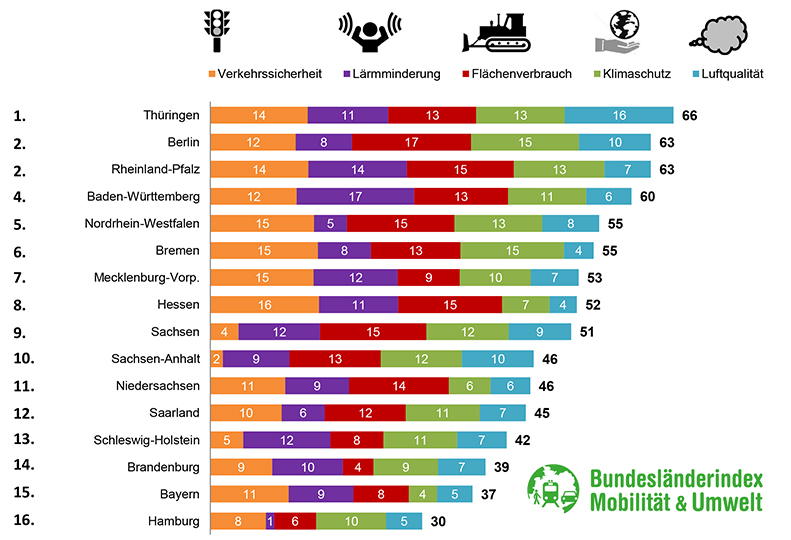
\includegraphics{​​​​../abbildungen/Mob-Index.jpg}
%\includegraphics[width=11cm]{abbildungen/mob-index} \\
\img{mob-index}{width=14cm}{Mobilitätsindex \footcite{Bundeslaenderindex:3}}
%\img{​​​​mob-index}​{​​​​width=11cm}​​​​{​​​​Mobilitätsindex}​​​​

%\cite{DUMMY:1}
%\footcite{Bundesländerindex:3}


\todo[inline]{QUELLE - EINBINDEN UND LINK \% https://www.allianz-pro-schiene.de/wp-content/uploads/2015/08/blimu-100.jpg}

"Fünf Themen fließen in das Gesamtergebnis ein: Verkehrssicherheit, Lärmminderung, Flächenverbrauch, Klimaschutz und Luftqualität."

\todo[inline]{PRÄZISIEREN !!! \% weiter ausführen und genauen Vergleich mit QUellen angeben}

Alle fünf Themen sind wichtig aber können keine Aussage zur Mobilität geben. Alleine das fehlen, des bereits erwähnten Gewichtes, der Durschnittsgeschwindigkeit lässt an der Gültigkeit und Aussagekraft eines Mobilitätsindexes zweifeln.
Deshalb sollte viel Kraft in die ausgewogene und gut gewichtete Gestaltung eines formalen allgemeingültigen Mobilitätsindexes gesetzt werden.

Auch die genutzten Quellen sollten nicht statisch sein sondern wie in dem Projekt dynamsich sein. Das ermöglicht ein ständig sich anpassendes Bild. Der Index lebt wie die Stadt bzw. der Raum selbst der bewertet werden soll.
